% !TeX root = ../main.tex
% Add the above to each chapter to make compiling the PDF easier in some editors.

\chapter{Variational Autoencoder}\label{chapter:vae}

Some text about generative models and variational autoencoder \parencite{VAE} in its original form being the chosen one.

\section{Architecture Search}
Searching for optimal hyperparamaters is a challenging task with many different approaches \parencite{HyperParameters}.
In particular, designing a good architecture takes a lot of trial and error.
Thus, different architectures are explored to determine a suitable one.
For this, first a basline architecture is established.
Then, different variations of this architecture are explored and trained.
The architecture of the model with the best performance is then chosen as the model architecture for this thesis.

Each variation is trained with for $20$ epochs on the TNO 2015 data only to decrease the architecture bias during search.
The dataset split is $t=0.15$, $v=0.15$, with the test set not being used at all.
The batch size is $32$.
As optimizer AmsGrad \parencite{AmsGrad} is used with a learning rate of $\dots$.
Gradients are clipped at $0.5$.
% Add any further hyperparameters.

\section{Baseline Architecture}
The baseline architecture is inspired by \parencite{Tightrope}.
This means that the bottleneckl layers have a high width and height.
As the input width and height of the emission fields are $32$ by $32$, the Bottleneck width and height are chosen as $8$ by $8$.
Inspired by \parencite{AllConvolutional} , to reduce the width and height dimensions, instead of using pooling operations, $2$ strided convolutions are used.
The strided convolutions, depicted in Figure, have kernel 2 and stride 2, thus halfing the size.

\begin{figure}[h!]
    \centering
    \begin{minipage}[b]{0.45\textwidth}
        \centering
        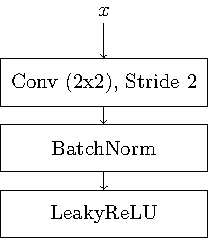
\includegraphics[]{figures/model_architecture/build/conv_layer.pdf}
        \caption{Conv Layer}
    \end{minipage}
    \hfill
    \begin{minipage}[b]{0.45\textwidth}
        \centering
        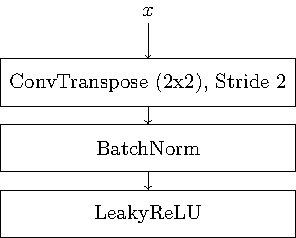
\includegraphics[]{figures/model_architecture/build/deconv_layer.pdf}
        \caption{DeConv Layer}
    \end{minipage}
\end{figure}

The strided convolution layers make use of the LeakyReLu activation function and batch normalization \parencite{BatchNorm}, as a regularization technique.

Vice versa, in the decoder, 2 strided transpose convolutions with the same parameters are used to double the width and height instead of upsampling layers.

In between the strided convolutions residual convolutional layers (ResConv) \parencite{ResNet} are used.
They can be seen in Figure.
\begin{figure}[h!]
    \centering
    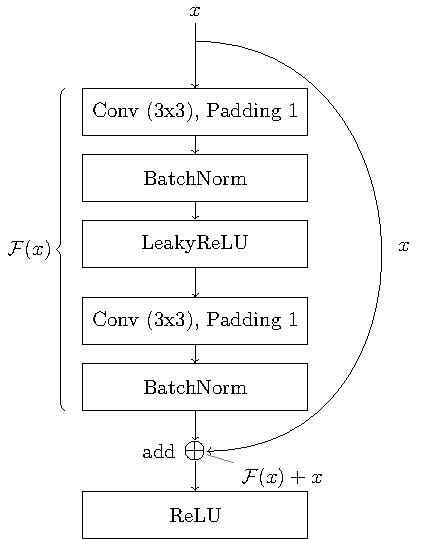
\includegraphics[]{figures/model_architecture/build/residual_conv_layer.pdf}
    \caption{ResConv Layer \parencite{ResNet}}
\end{figure}
The ResConv layers make use of two convolutions with kernel 3 and padding 1 to retain the width and height dimensions.
The output activation is ReLu.
In between the two convolutional layers, LeakyReLu is used again.
Again, batchnorm is applied.
\begin{figure}[h!]
    \centering
    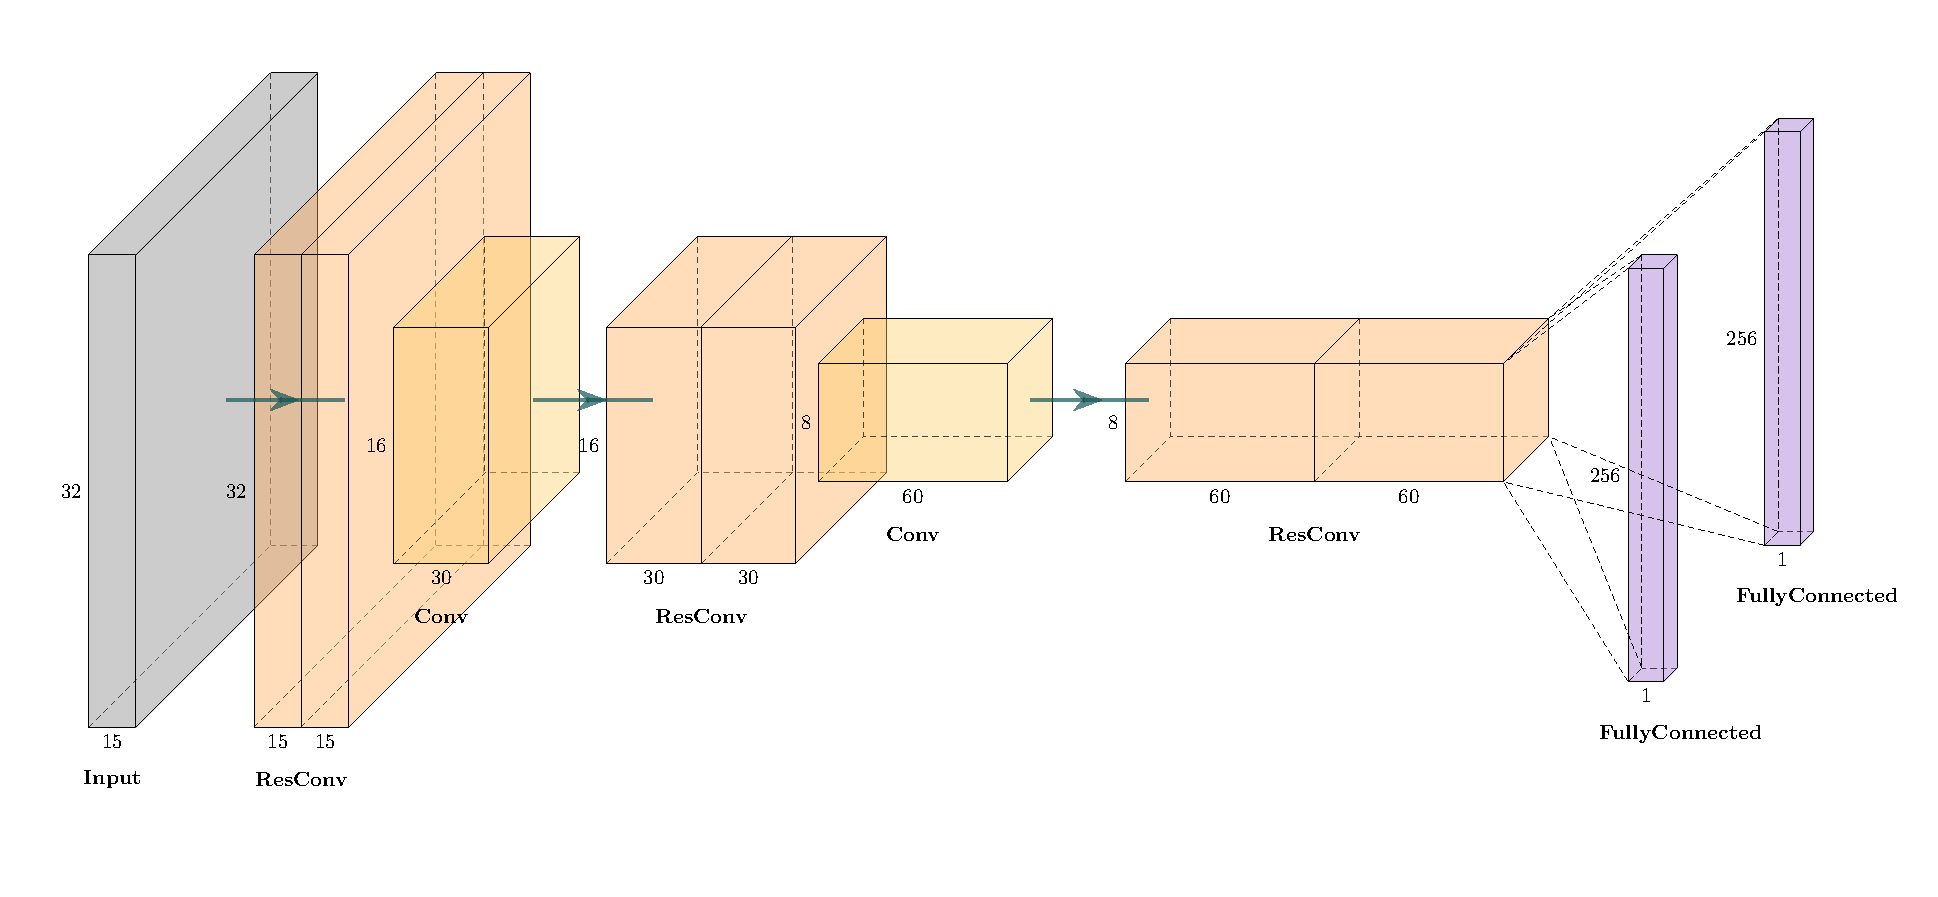
\includegraphics[width=\textwidth]{figures/model_architecture/build/baseline_vae_encoder.pdf}
    \caption{Baseline Encoder Architecture (generated with \parencite{NNVisualization})}
\end{figure}
\begin{figure}[h!]
    \centering
    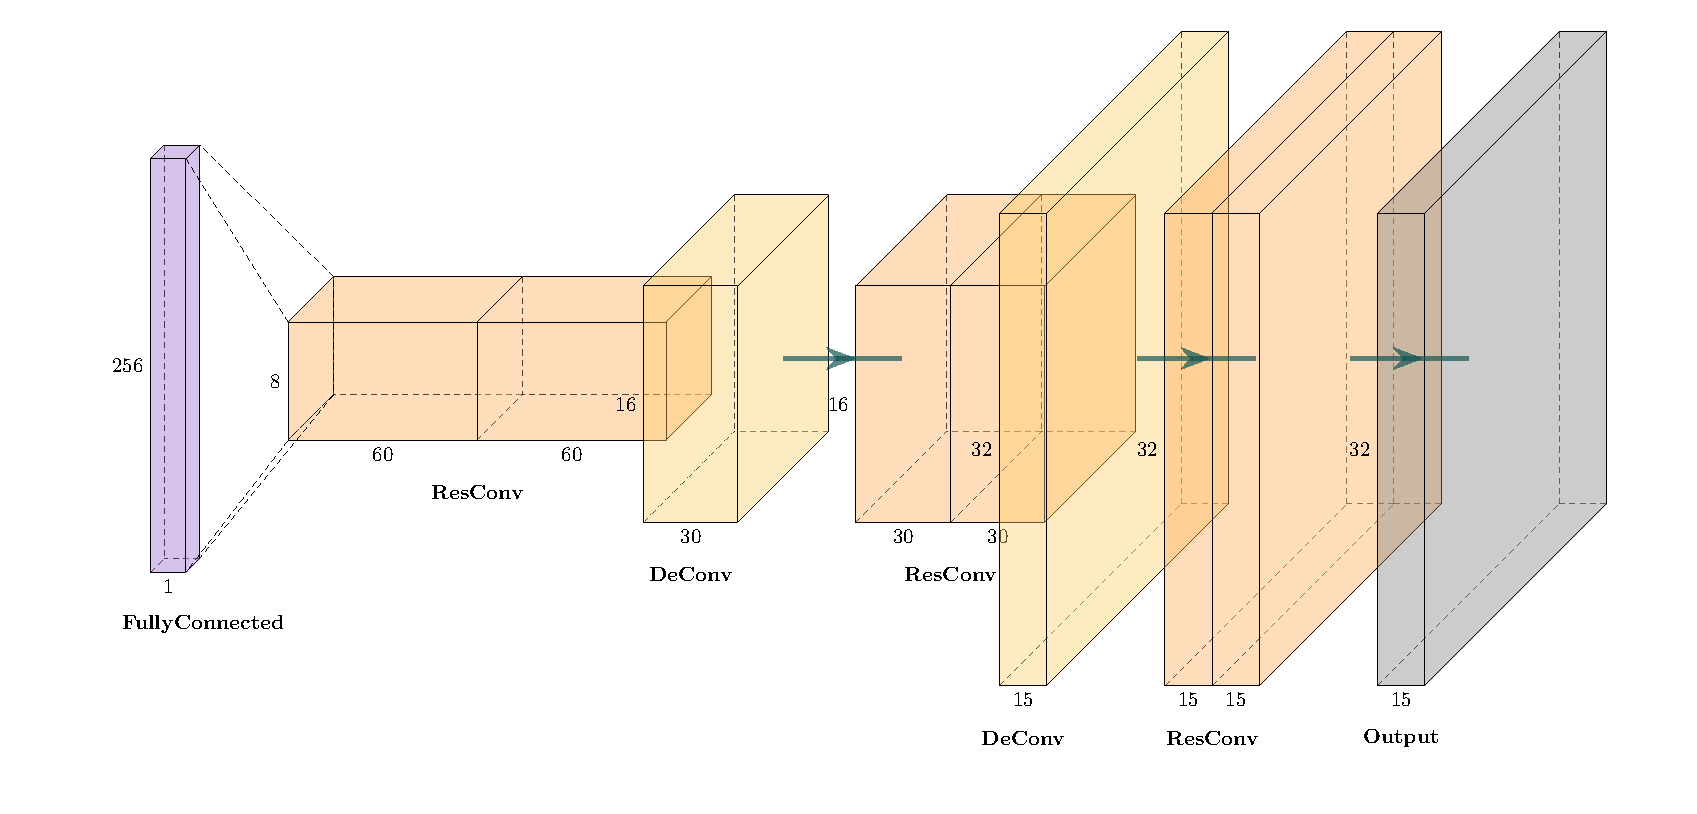
\includegraphics[width=\textwidth]{figures/model_architecture/build/baseline_vae_decoder.pdf}
    \caption{Baseline Decoder Architecture (generated with \parencite{NNVisualization})}
\end{figure}
As can be seen in Figure and Figure, the 2 strided convolutions are located between $2$ layers of ResConv layers each, in the encoder and decoder.
Fully connected layers are used at the end of the encoder and beginning of the decoder to achive a hidden dimension $256$ of the latent space. 
The last ResConv layers does not use batch normalization.
The number of parameters is \dots.

The loss function used is the typical VAE loss with MSE loss as recontruction loss and Elbo \parencite{VAE} \dots .
\begin{equation}
    L(x, \hat{x}) = 1 + 2
\end{equation}
In addition to the loss, at each step the SSIM \parencite{SSIM} is computed as it provides qualitatively better comparison between two emission fields than the MSE as it takes structure into account.

\section{Explored Variations}
The following variations are explored
\begin{enumerate}
    \item conv layers to increase / decrease depth and pooling layers to decrease width/height and upsample layers to increase width/height
    \item upsampling emission fields to $64$ by $64$ and then applying convlutions; in decoder max pooling to downsample $64$ by $64$ to $32$ by $32$
    \item more depth; instead of doubling depth, quadrupling it
    \item 2 conv layers for changing width and height instead of one strided convolution
    \item 3 ResConv layers everywhere
    \item residual layers with identity mappings depicted in Figure based on \parencite{IdentityMappings} instead of ResConv layers from Figure
    \item residual layers with identity mappings with dropout \parencite{Dropout} based on \parencite{WideResNet} (add explanation)
\end{enumerate}

\begin{figure}[h!]
    \centering
    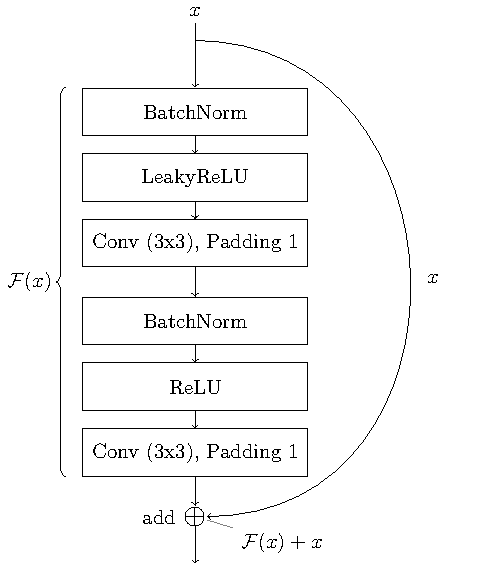
\includegraphics[]{figures/model_architecture/build/residual_conv_with_im_layer.pdf}
    \caption{ResConv Layer With Identity Mappings \parencite{IdentityMappings}}
\end{figure}

In Figure , the validation losses and validation SSIM can be seen from the 20 epoch trianing runs.

\begin{figure}
    \centering
    \begin{subfigure}{.5\textwidth}
        \centering
        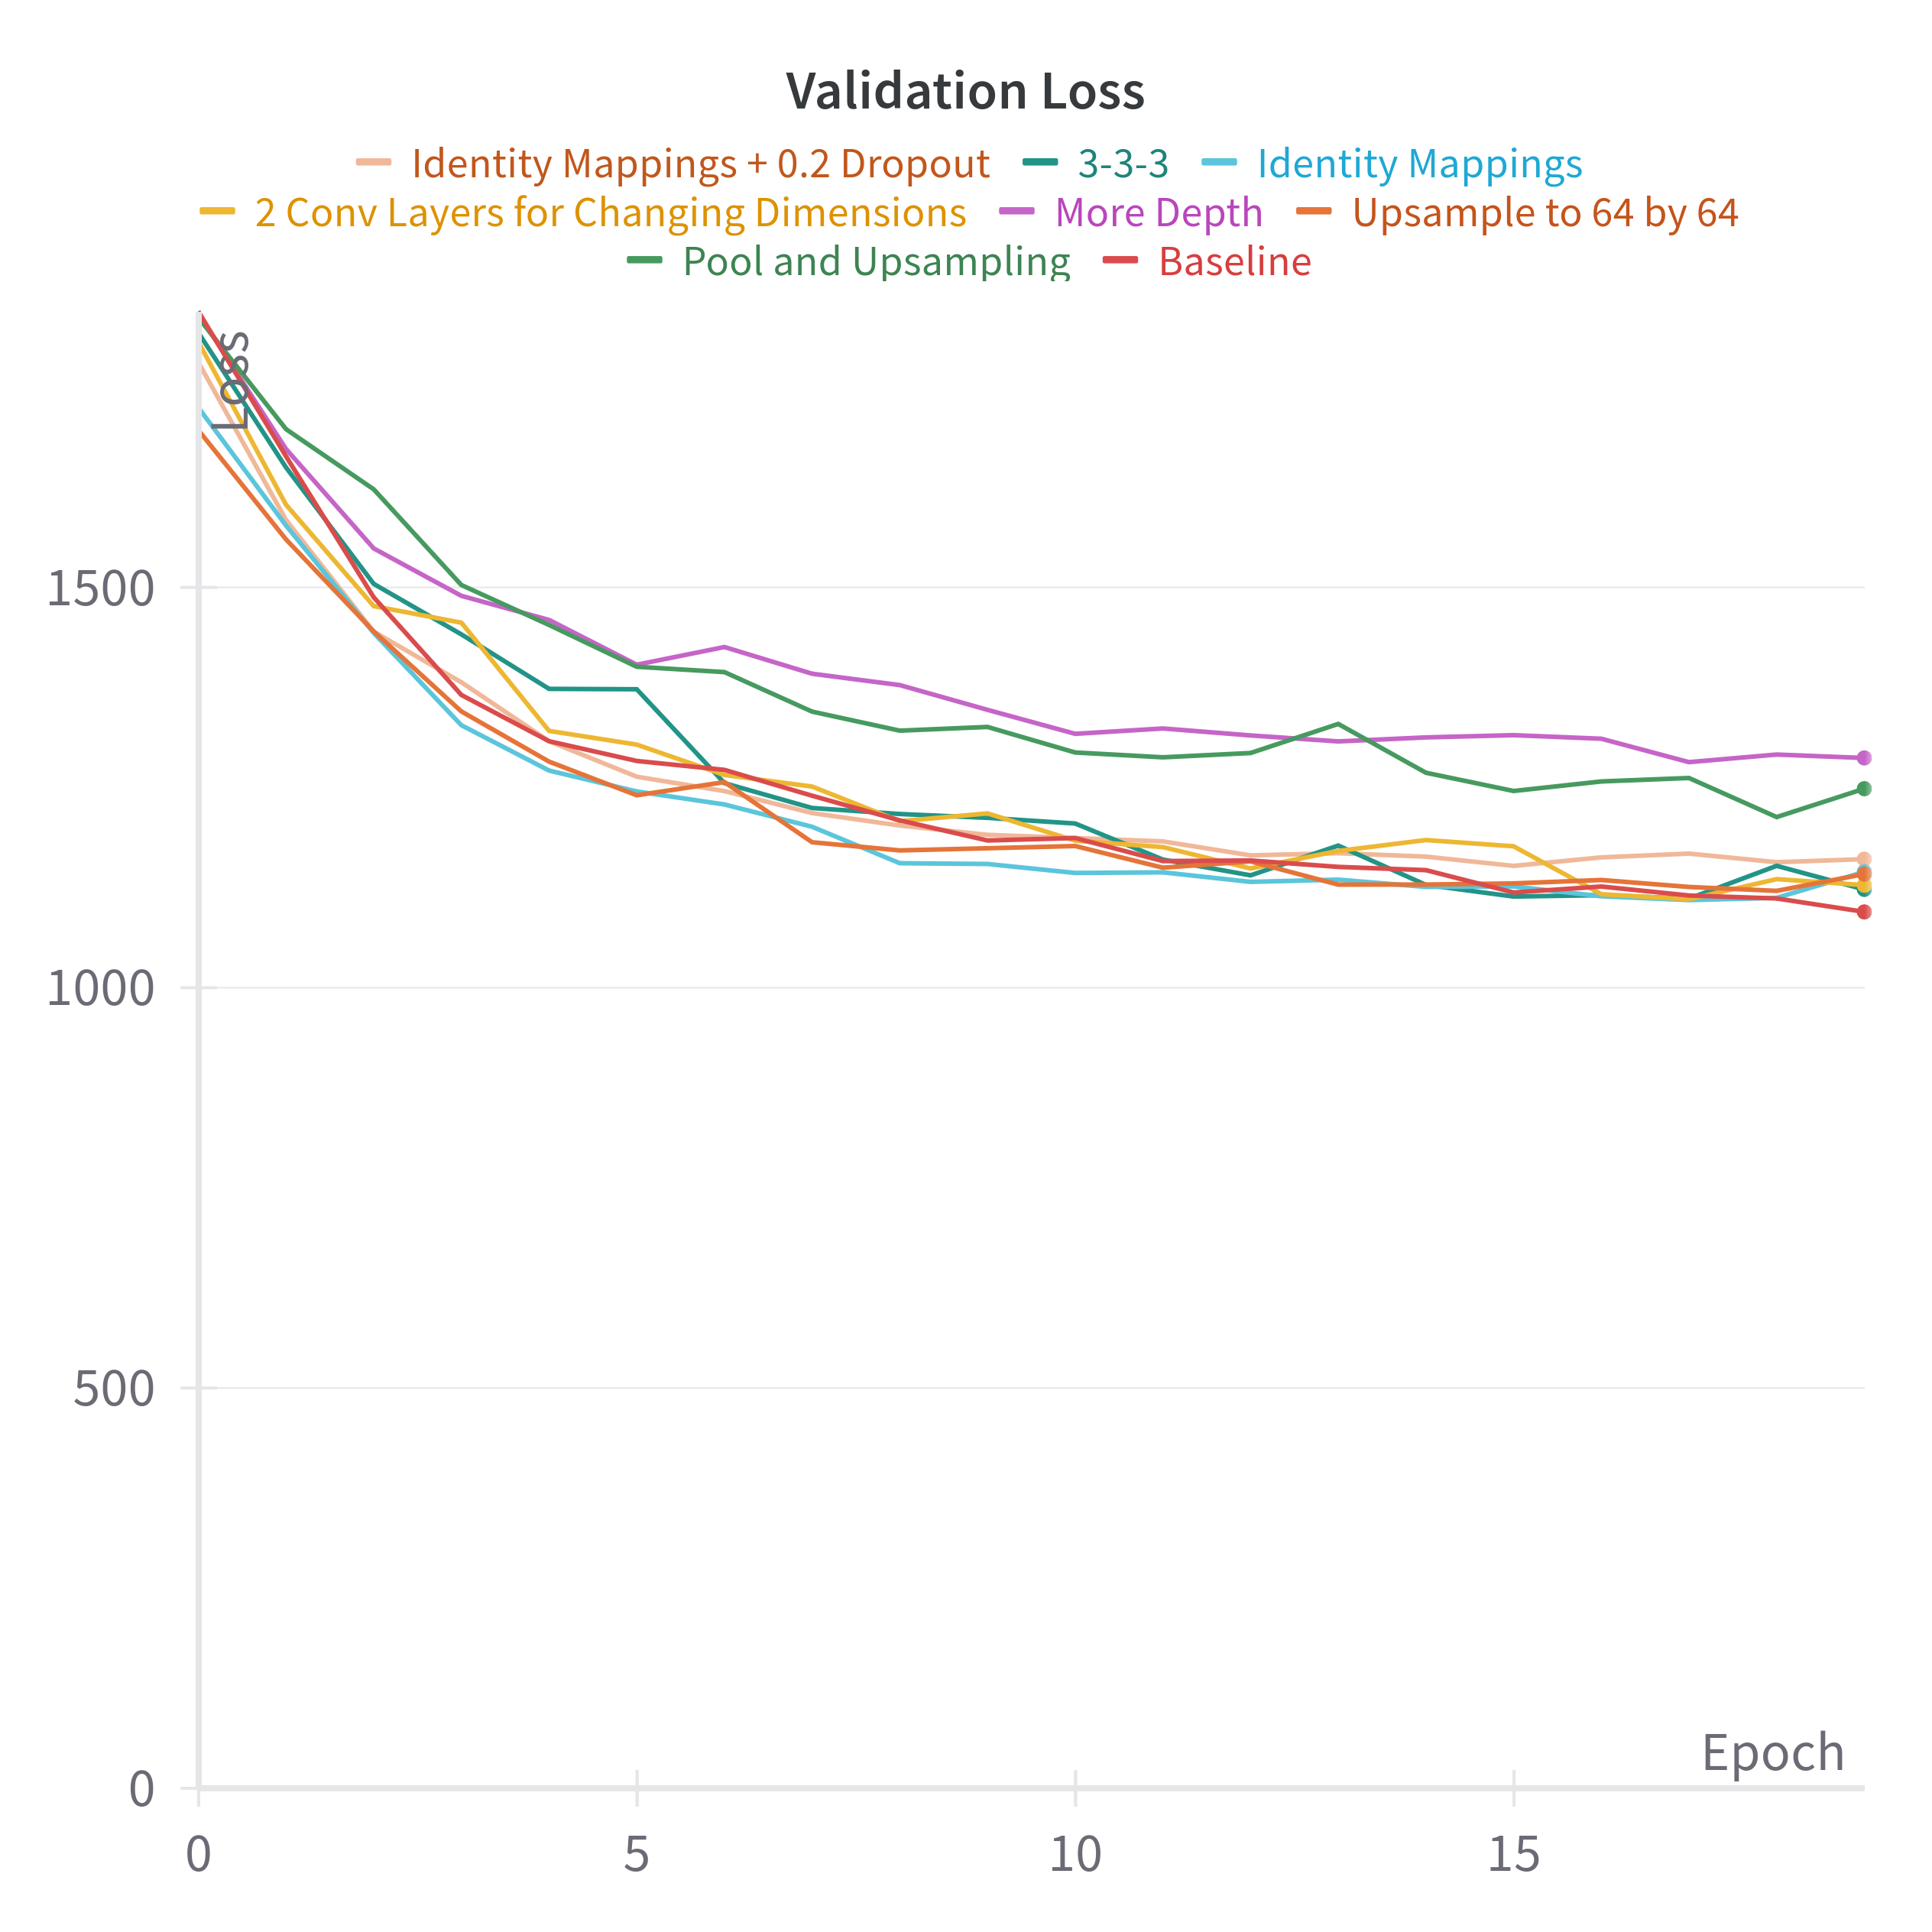
\includegraphics[width=\linewidth]{figures/architecture_variations/validations_loss.png}
        \caption{Validation Loss}
        \label{fig:sub1}
    \end{subfigure}%
    \begin{subfigure}{.5\textwidth}
        \centering
        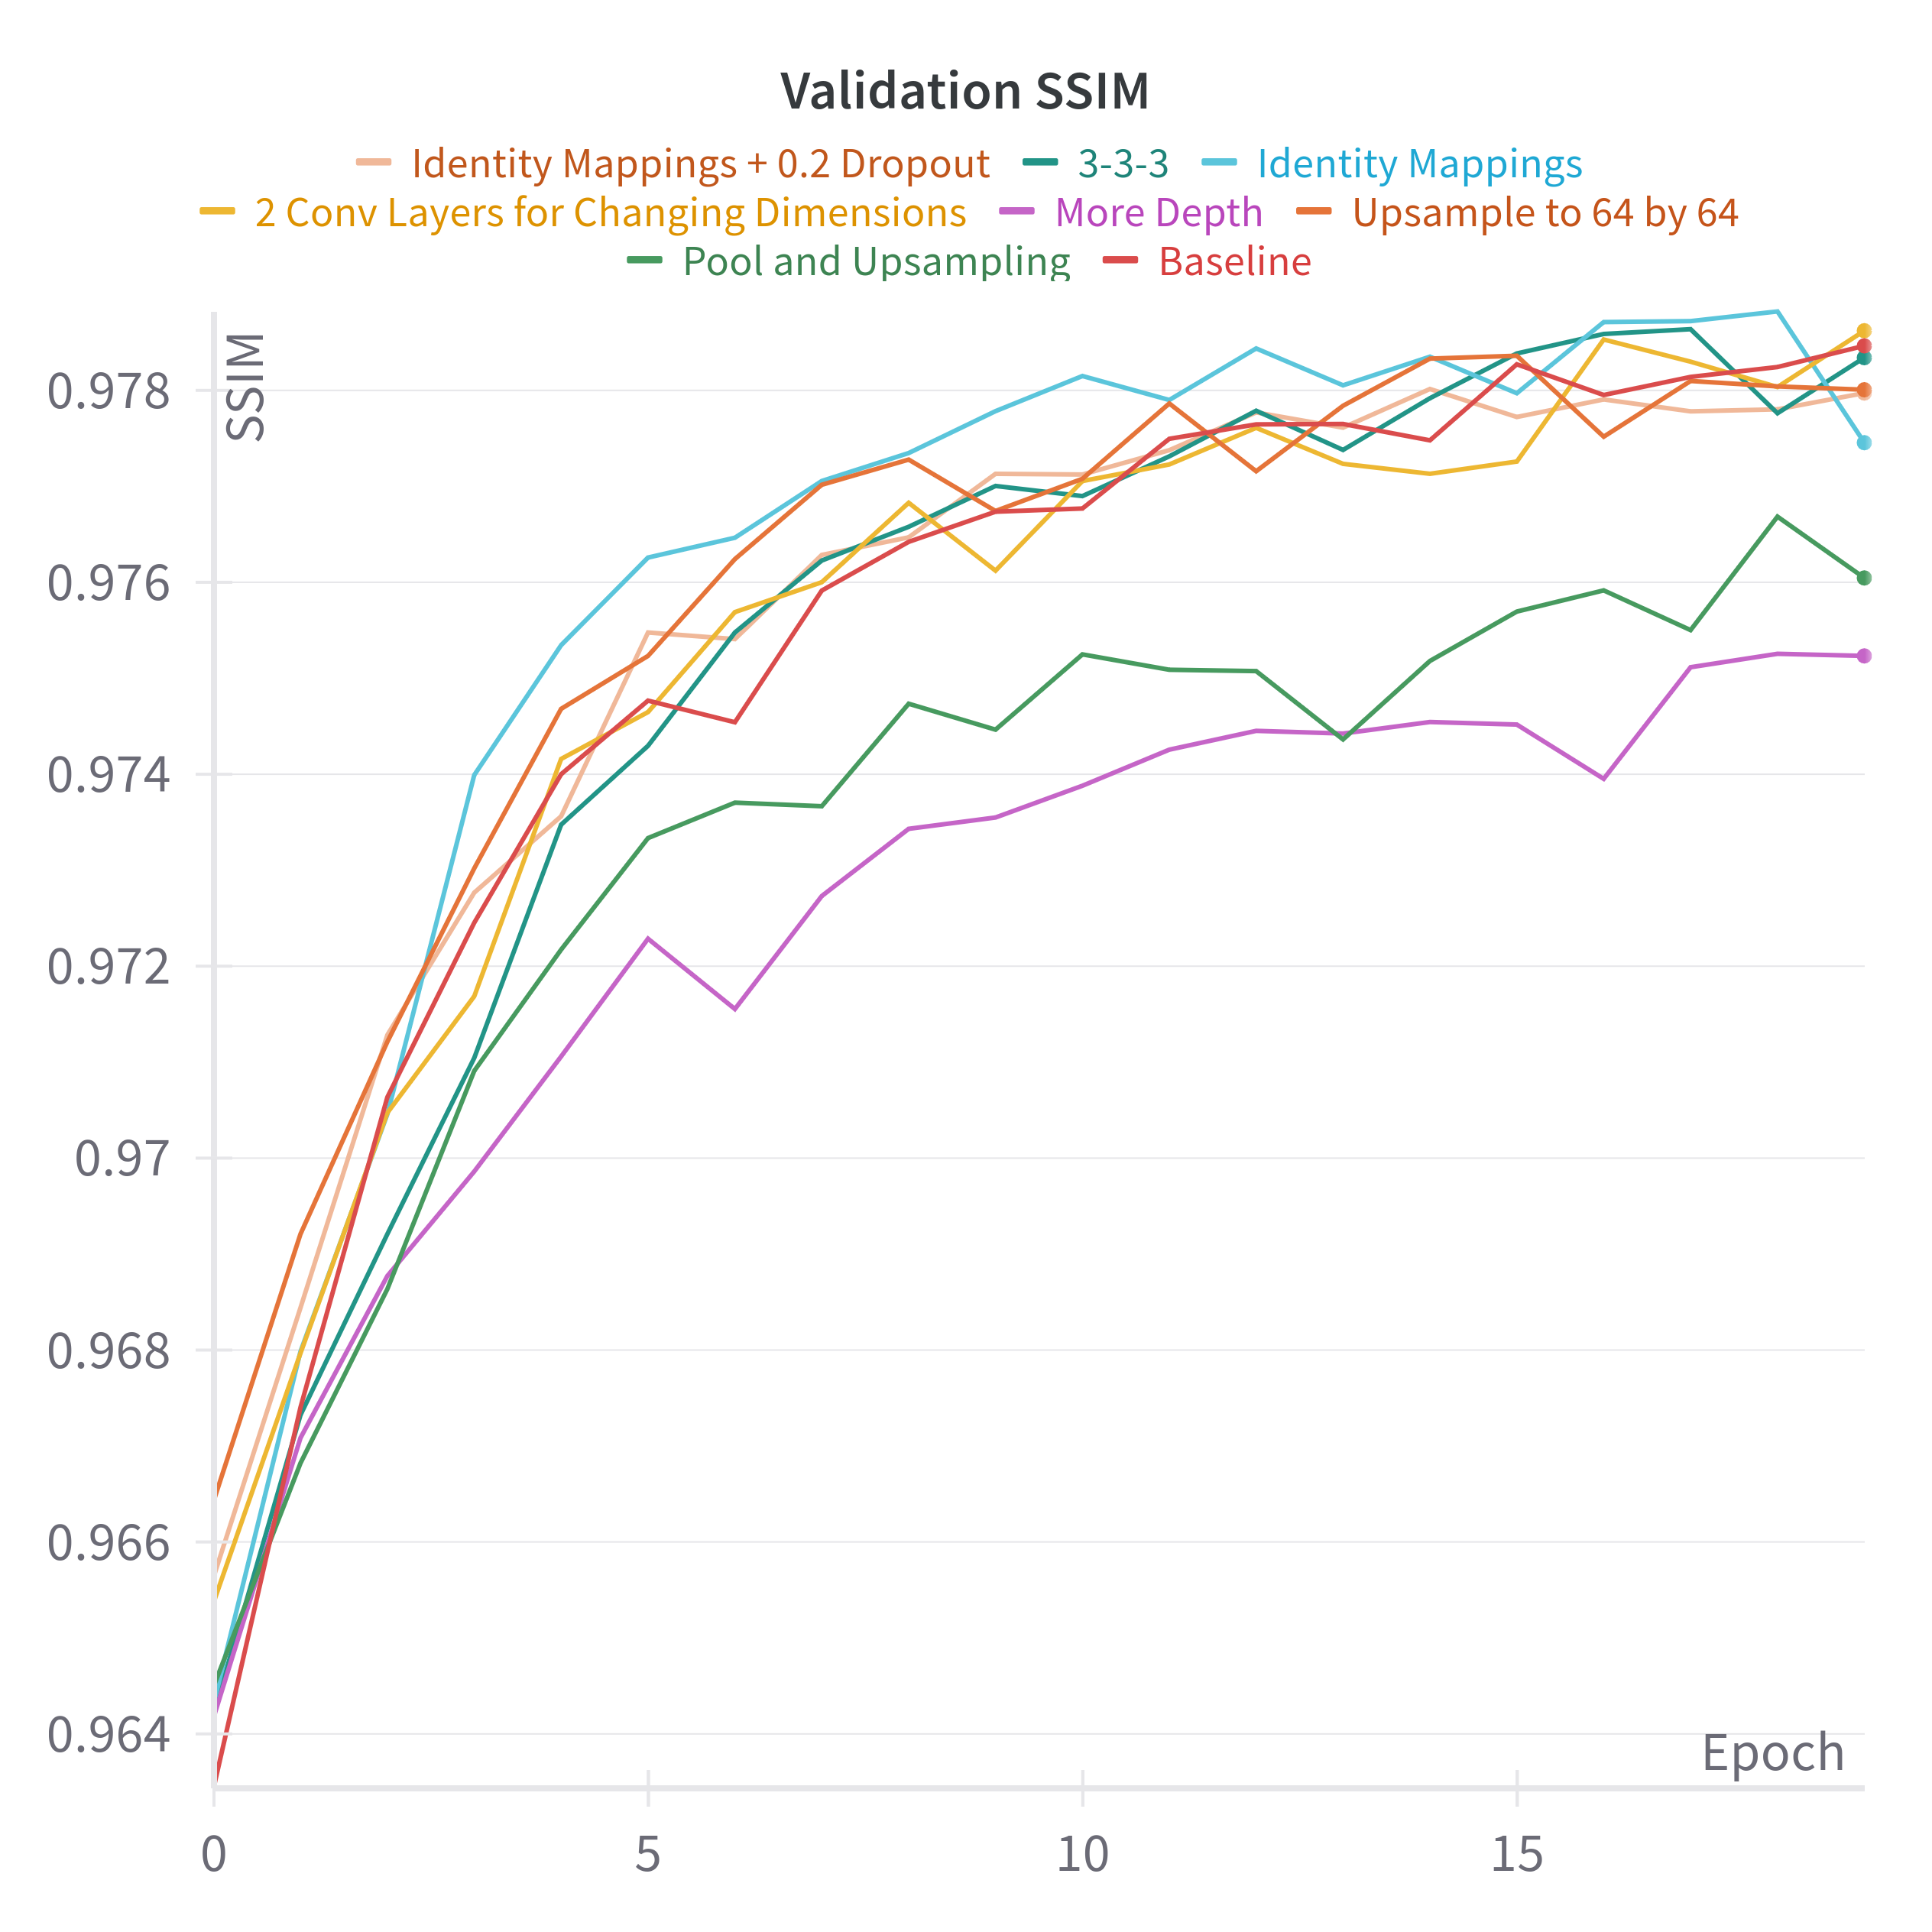
\includegraphics[width=\linewidth]{figures/architecture_variations/validation_ssim.png}
        \caption{Validation SSIM}
        \label{fig:sub2}
    \end{subfigure}
    \caption{Performance of Variations on Validation Data During Training}
    \label{fig:test}
\end{figure}

Add some observations.

\section{Final Architecture}
From the previous subsection, it can be concluded that the baseline architecture performs very well.
The following changes are made to result in the final architecture.
First, the residual layers in Figure  with identity mappings are used.
Furthermore, they are extended with dropout as proposed in \parencite{WideResNet} in the \dots.
Finally, the number of residual layers are increased to $3$.
The encoder and decoder respectively can be seen in Figure and Figure.
\begin{figure}[h!]
    \centering
    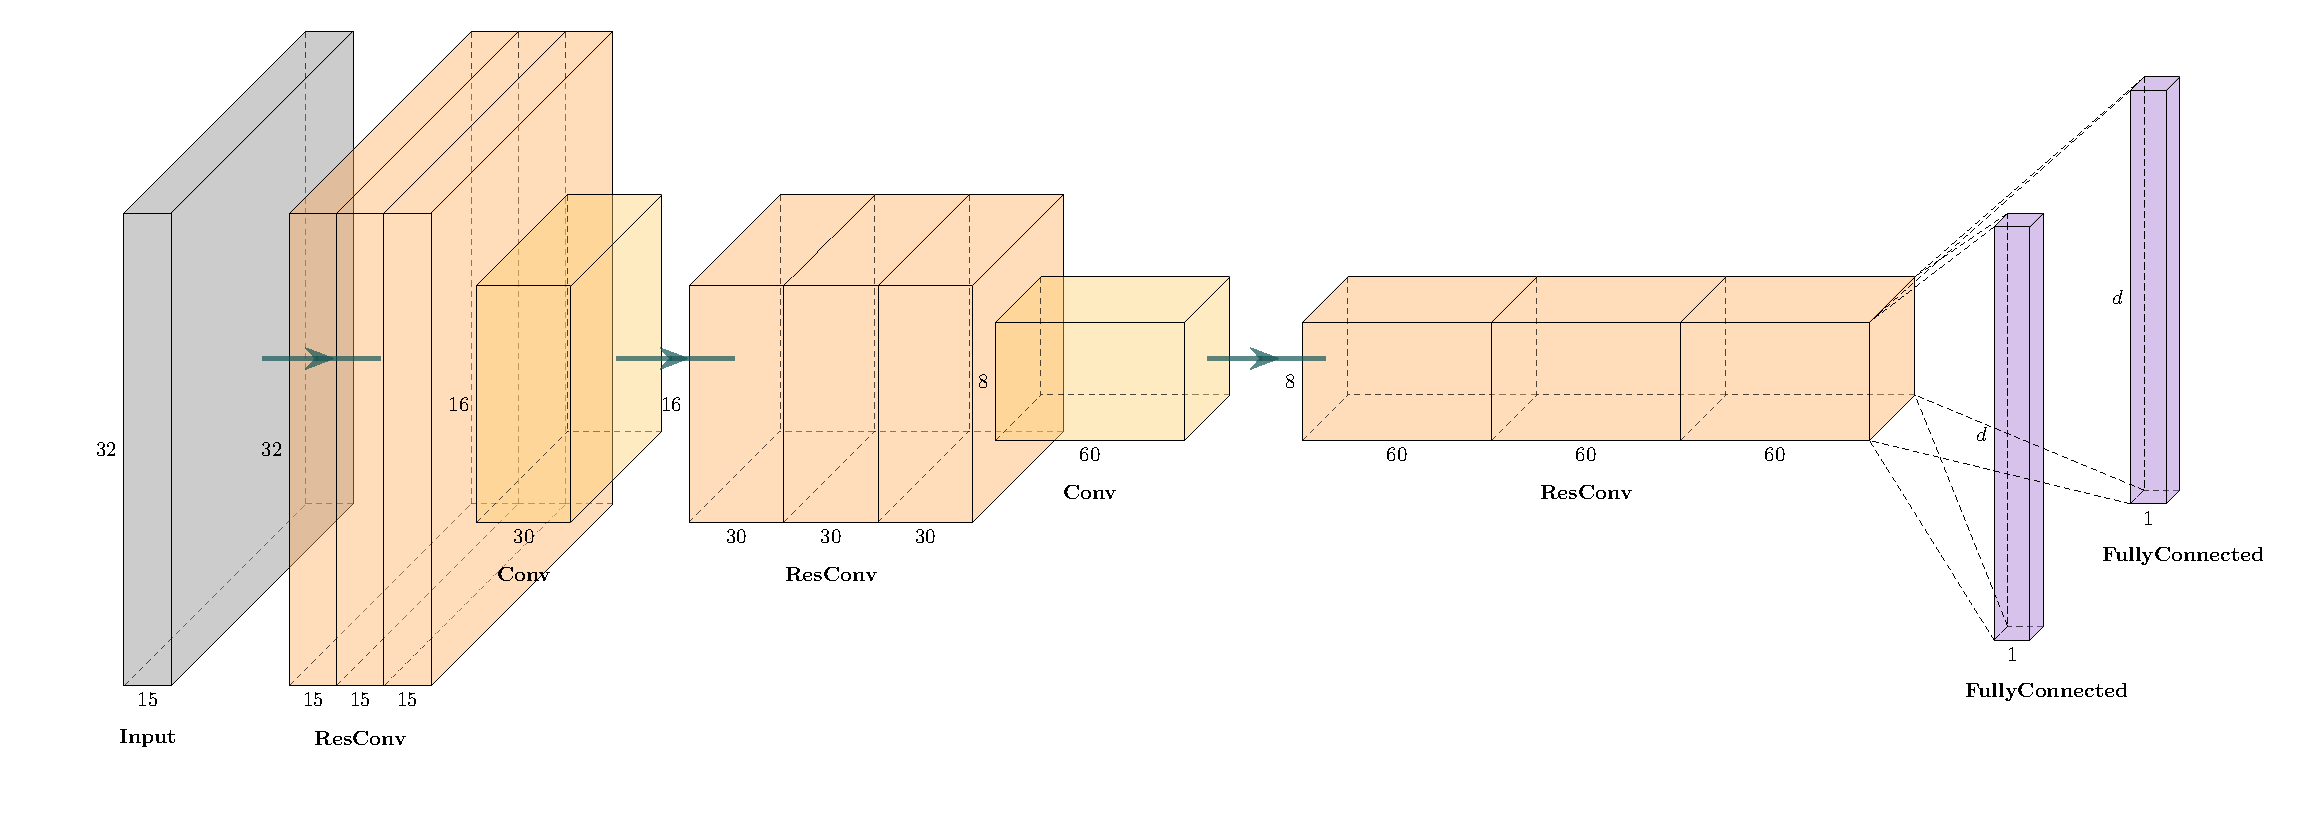
\includegraphics[width=\textwidth]{figures/model_architecture/build/final_vae_encoder.pdf}
    \caption{Final Encoder Architecture (generated with \parencite{NNVisualization})}
\end{figure}
\begin{figure}[h!]
    \centering
    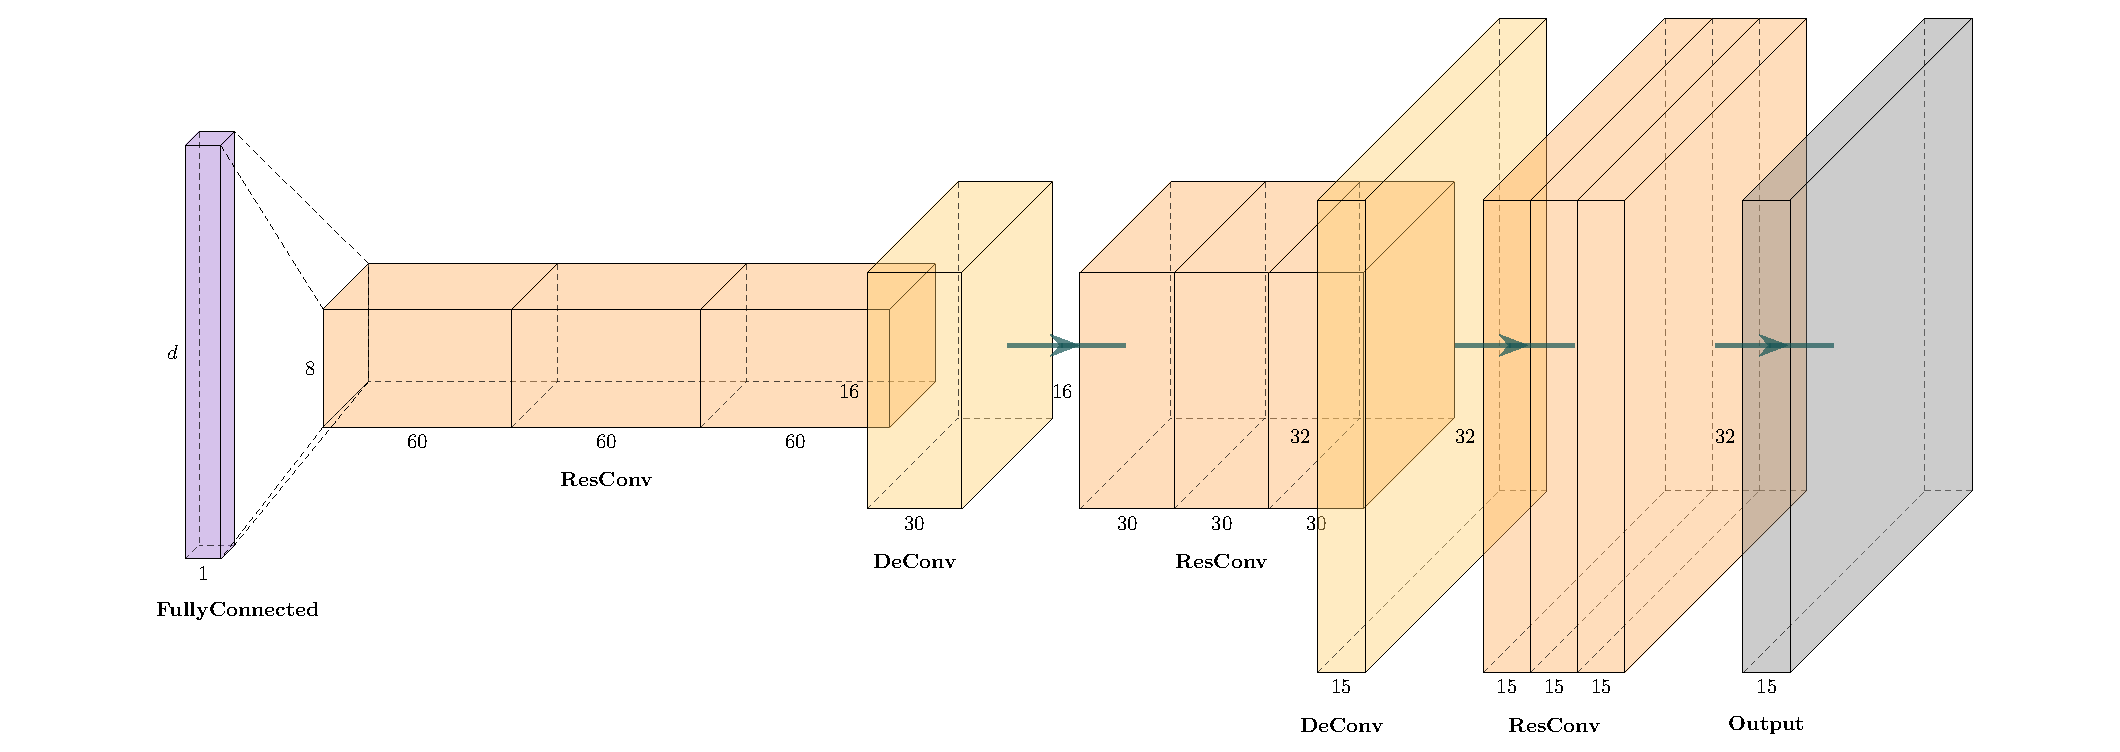
\includegraphics[width=\textwidth]{figures/model_architecture/build/final_vae_decoder.pdf}
    \caption{Final Decoder Architecture (generated with \parencite{NNVisualization})}
\end{figure}
The latent dimension $d$ which was kept at $d = 256$ for the "ablation study" is now kept parametrizable.
In fact, for this thesis, different latent dimensions are explored: $d \in {256, 512, 1024, 2048}$.
The number of parameters of the model in dependence of $d$ are \dots.

The models are trained on both the TNO 2015 and 2018 data for $100$ epochs.
The dataset split is $t = 0.13$ and $v = 0.15$, resulting in $13$ cities in the test, $15$ cities in the validation, and $74$ cities in the training set.
The exact split can be seen in appendix \dots.
The weights of the model with the highest validation SSIM during the $100$ epochs is stored.
All other relevant hyperparamaters are kept the same as in the the variations subsection.

The training losses, SSIM, and mean MSE can be seen in Figure for each $d$.
(add Figure).
It can be observed that there is overfitting present in the data.
This may be related to samples like London or Berlin in the trianing data that steer the loss, resulting in overfitting to these cities, due to their size of emissions.
The amount of overfitting decreases with an increase in $d$.


\section{Fine-tuning}
Fine-tuning is a popular technique to steer a model to do somthing more specific \cite{FineTuning}.
In the case of this thesis, fine-tuning the trained model to specific cities may make sense to achieve more precise recontruction.
The idea is that a generative model can learn the structure of the city and focus on differences of emissions due to observed data.
Thus, fine-tuning is evaluated in this thesis.
For this, the three for the case studies chosen cities are used.

During fine-tuning, the weights of the original models are updated.
The learning rate is reduced.
In our case, we chose $1e-x$ as learning rate.

For fine-tuning, the TNO 2015 data is used.
Later, for evaluation the TNO 2018 is used.

To prevent the model from overfitting to the 2015 data and train the model to generalize to unknown emitters, i.e. during the bottom up estimations, the following things are done \dots.


